\documentclass[border=6pt]{standalone}
\usepackage{fontspec}
\setmainfont{TeX Gyre Termes}
\usepackage{tikz}
\usetikzlibrary{arrows.meta,positioning,fit,backgrounds}
\definecolor{navy}{HTML}{16324F}
\definecolor{blue}{HTML}{2F6690}
\definecolor{green}{HTML}{3A7D44}
\definecolor{orange}{HTML}{D17A22}
\definecolor{red}{HTML}{A23E48}
\definecolor{lightblue}{HTML}{EAF3F8}
\definecolor{lightgreen}{HTML}{EAF5EC}
\definecolor{lightorange}{HTML}{FFF2DF}
\definecolor{lightred}{HTML}{FBEAEC}
\tikzset{
  box/.style={draw=navy, very thick, rounded corners=2pt, align=center, font=\small, inner sep=5pt, minimum height=0.9cm},
  data/.style={box, fill=lightblue, text width=2.25cm},
  calc/.style={box, fill=lightgreen, text width=2.25cm},
  agent/.style={box, fill=lightorange, text width=2.5cm},
  control/.style={box, fill=lightred, text width=2.5cm},
  arrow/.style={-{Latex[length=2.5mm]}, very thick, draw=navy},
  danger/.style={-{Latex[length=2.5mm]}, very thick, draw=red, dashed},
  label/.style={font=\scriptsize, align=center, fill=white, inner sep=2pt},
  participant/.style={box, fill=lightblue, text width=2.3cm, minimum height=0.75cm},
  zone/.style={box, minimum height=1.1cm, text width=4.1cm},
  smallbox/.style={box, font=\scriptsize, text width=3.5cm, minimum height=0.7cm}
}

\begin{document}
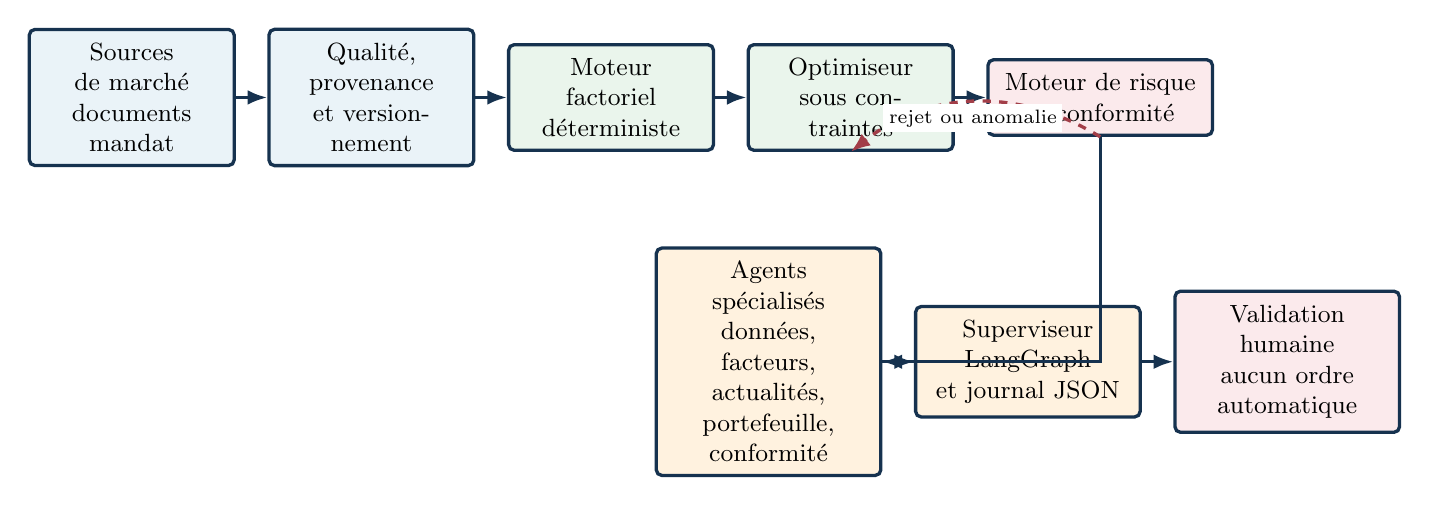
\begin{tikzpicture}[node distance=5mm and 4mm]
\node[data] (data) {Sources de marché\\documents\\mandat};
\node[data, right=of data] (quality) {Qualité, provenance\\et versionnement};
\node[calc, right=of quality] (factor) {Moteur factoriel\\déterministe};
\node[calc, right=of factor] (optimizer) {Optimiseur\\sous contraintes};
\node[control, right=of optimizer] (risk) {Moteur de risque\\et conformité};
\node[agent, below=12mm of factor, xshift=20mm] (agents) {Agents spécialisés\\données, facteurs, actualités,\\portefeuille, conformité};
\node[agent, right=of agents] (supervisor) {Superviseur\\LangGraph\\et journal JSON};
\node[control, right=of supervisor] (human) {Validation humaine\\aucun ordre\\automatique};
\draw[arrow] (data) -- (quality);
\draw[arrow] (quality) -- (factor);
\draw[arrow] (factor) -- (optimizer);
\draw[arrow] (optimizer) -- (risk);
\draw[arrow] (risk.south) |- (agents.east);
\draw[arrow] (agents) -- (supervisor);
\draw[arrow] (supervisor) -- (human);
\draw[danger] (risk.south) to[bend right=35] node[label,below]{rejet ou anomalie} (optimizer.south);
\end{tikzpicture}
\end{document}
